%% Author_tex.tex
%% V1.0
%% 2012/13/12
%% developed by Techset
%%
%% This file describes the coding for rsproca.cls

\documentclass[openacc]{rsproca_new}%%%%where rsproca is the template name
\usepackage{subcaption}
\usepackage[thinc]{esdiff} % for derivatives
\usepackage{empheq} % boxed equations
\usepackage{amsmath}
%\usepackage[section]{placeins}


\definecolor{myboxcolor}{rgb}{0.96, 0.96, 0.96}
\newcommand*\mybox[1]{%
\colorbox{myboxcolor}{\hspace{1em}#1\hspace{1em}}}

\usepackage{xspace}
\newcommand\thedata {$\{(t_i,h_{\text{obs}, i})\}_{i=1}^{N}$\xspace}
\newcommand\thedatanomath {\{(t_i,h_{\text{obs}, i})\}_{i=1}^{N}}
\newcommand\themodel {$h(t; h_0, \boldsymbol \alpha, \boldsymbol\theta)$\xspace}
\newcommand\themodelnomath {h(t; h_0, \boldsymbol \alpha, \boldsymbol\theta)}
\newcommand\thevars{h_0, \boldsymbol \alpha, \boldsymbol \theta, \sigma^2}
\newcommand\thesamples{$(h_{0, i}, \boldsymbol \alpha_i, \boldsymbol \theta_i, \sigma_i^2)_{i=1}^{N_s}$}



% from empheq pkg
\definecolor{shadecolor}{rgb}{0.97, 0.97, 1.0}
\definecolor{titlecolor}{rgb}{0.96, 1.0, 0.98}
\newsavebox{\mysaveboxM} % M for math
\newsavebox{\mysaveboxT} % T for text
\newcommand*\Garybox[2][Example]{%
\sbox{\mysaveboxM}{#2}%
\sbox{\mysaveboxT}{\fcolorbox{black}{titlecolor}{#1}}%
\sbox{\mysaveboxM}{%
\fcolorbox{black}{shadecolor}{%
\makebox[\linewidth-10em]{\usebox{\mysaveboxM}}%
}%
}%
\usebox{\mysaveboxM}%
\makebox[0pt][r]{%
\makebox[\wd\mysaveboxM][c]{%
\raisebox{\ht\mysaveboxM-0.5\ht\mysaveboxT
+1.6\dp\mysaveboxT-0.5\fboxrule}{\usebox{\mysaveboxT}}%
}%
}%
}


\usepackage{tcolorbox} 
\tcbuselibrary{breakable}
\newtcolorbox[auto counter
]{mytcbox}[2][]{
% title=Box~\thetcbcounter: #2,#1,
title=#2, #1,
colback=white,
colframe=black,
fonttitle=\bfseries,
parbox=false
}


%%%% *** Do not adjust lengths that control margins, column widths, etc. ***

%%%%%%%%%%% Defining Enunciations  %%%%%%%%%%%
\newtheorem{theorem}{\bf Theorem}[section]
\newtheorem{condition}{\bf Condition}[section]
\newtheorem{corollary}{\bf Corollary}[section]
%%%%%%%%%%%%%%%%%%%%%%%%%%%%%%%%%%%%%%%%%%%%%%%

%%%%% Please insert respective article type here %%%%
\titlehead{Research}

\begin{document}

%%%% Article title to be placed here
% \title{Bayesian inference of the shape of an object inside of a gravity-drained tank}
%\title{Inferring the shape of a solid inside a gravity-drained tank from liquid level time series data}
\title{Inferring the shape of a solid inside a liquid-holding tank from its liquid level as it drains}


\author{%%%% Author details
Gbenga Fabusola$^{1}$, 
Cory M. Simon$^{1}$
}

%%%%%%%%% Insert author address here
\address{$^{1}$School of Chemical, Biological, and Environmental Engineering. Oregon State University. Corvallis, OR, USA.
% $^{2}$Second author address\\
}

%%%% Subject entries to be placed here %%%%
\subject{applied mathematics, chemical engineering}

%%%% Keyword entries to be placed here %%%%
\keywords{inverse problems, Bayesian statistical inversion, Torricelli's law}

%%%% Insert corresponding author and its email address}
\corres{Cory M. Simon\\
\email{cory.simon@oregonstate.edu}}

%%%% Abstract text to be placed here %%%%%%%%%%%%
\begin{abstract}
In engineering, we often encounter an open-top, liquid-holding tank draining via gravity-driven flow through a small orifice in its side. 
Torricelli's law and a mass balance give a differential equation model governing the dynamics of the liquid level in the tank. 
Herein, we consider the inverse problem of leveraging this model to infer the shape of an exogenous solid, heavy object inside of a tank draining of liquid, using measurements of the liquid level over time. (Because the object displaces liquid, the rate of decrease of the liquid level provides information about the cross-sectional area of the object at that height; as the liquid level drops, we ``scan'' the area of the object as a function of height.) To quantify uncertainty about the shape of the object, we employ Bayesian statistical inversion for reconstructing the object's cross-sectional area as a function of height. 

In our experimental setup, a small, open-top tank 
% (an inverted, truncated cone with a rounded rectangle base) 
drains of water through a small orifice in its side; a liquid level sensor collects time series data of the water level. 
First, we calibrate and test our forward model of the dynamics of the water level using data from two drainage experiments without an object inside of the tank. Second, we conduct a drainage experiment with an object inside the tank, then leverage the calibrated forward model and the liquid level time series data to predict (i.e., obtain a posterior distribution for) the shape of the object inside the tank with quantified uncertainty.
Our approach may be practically useful to infer the shape of an unknown object, or the porosity of packed particles, inside of an opaque tank that gives access to liquid level measurements. 
\newline

\begin{center}
	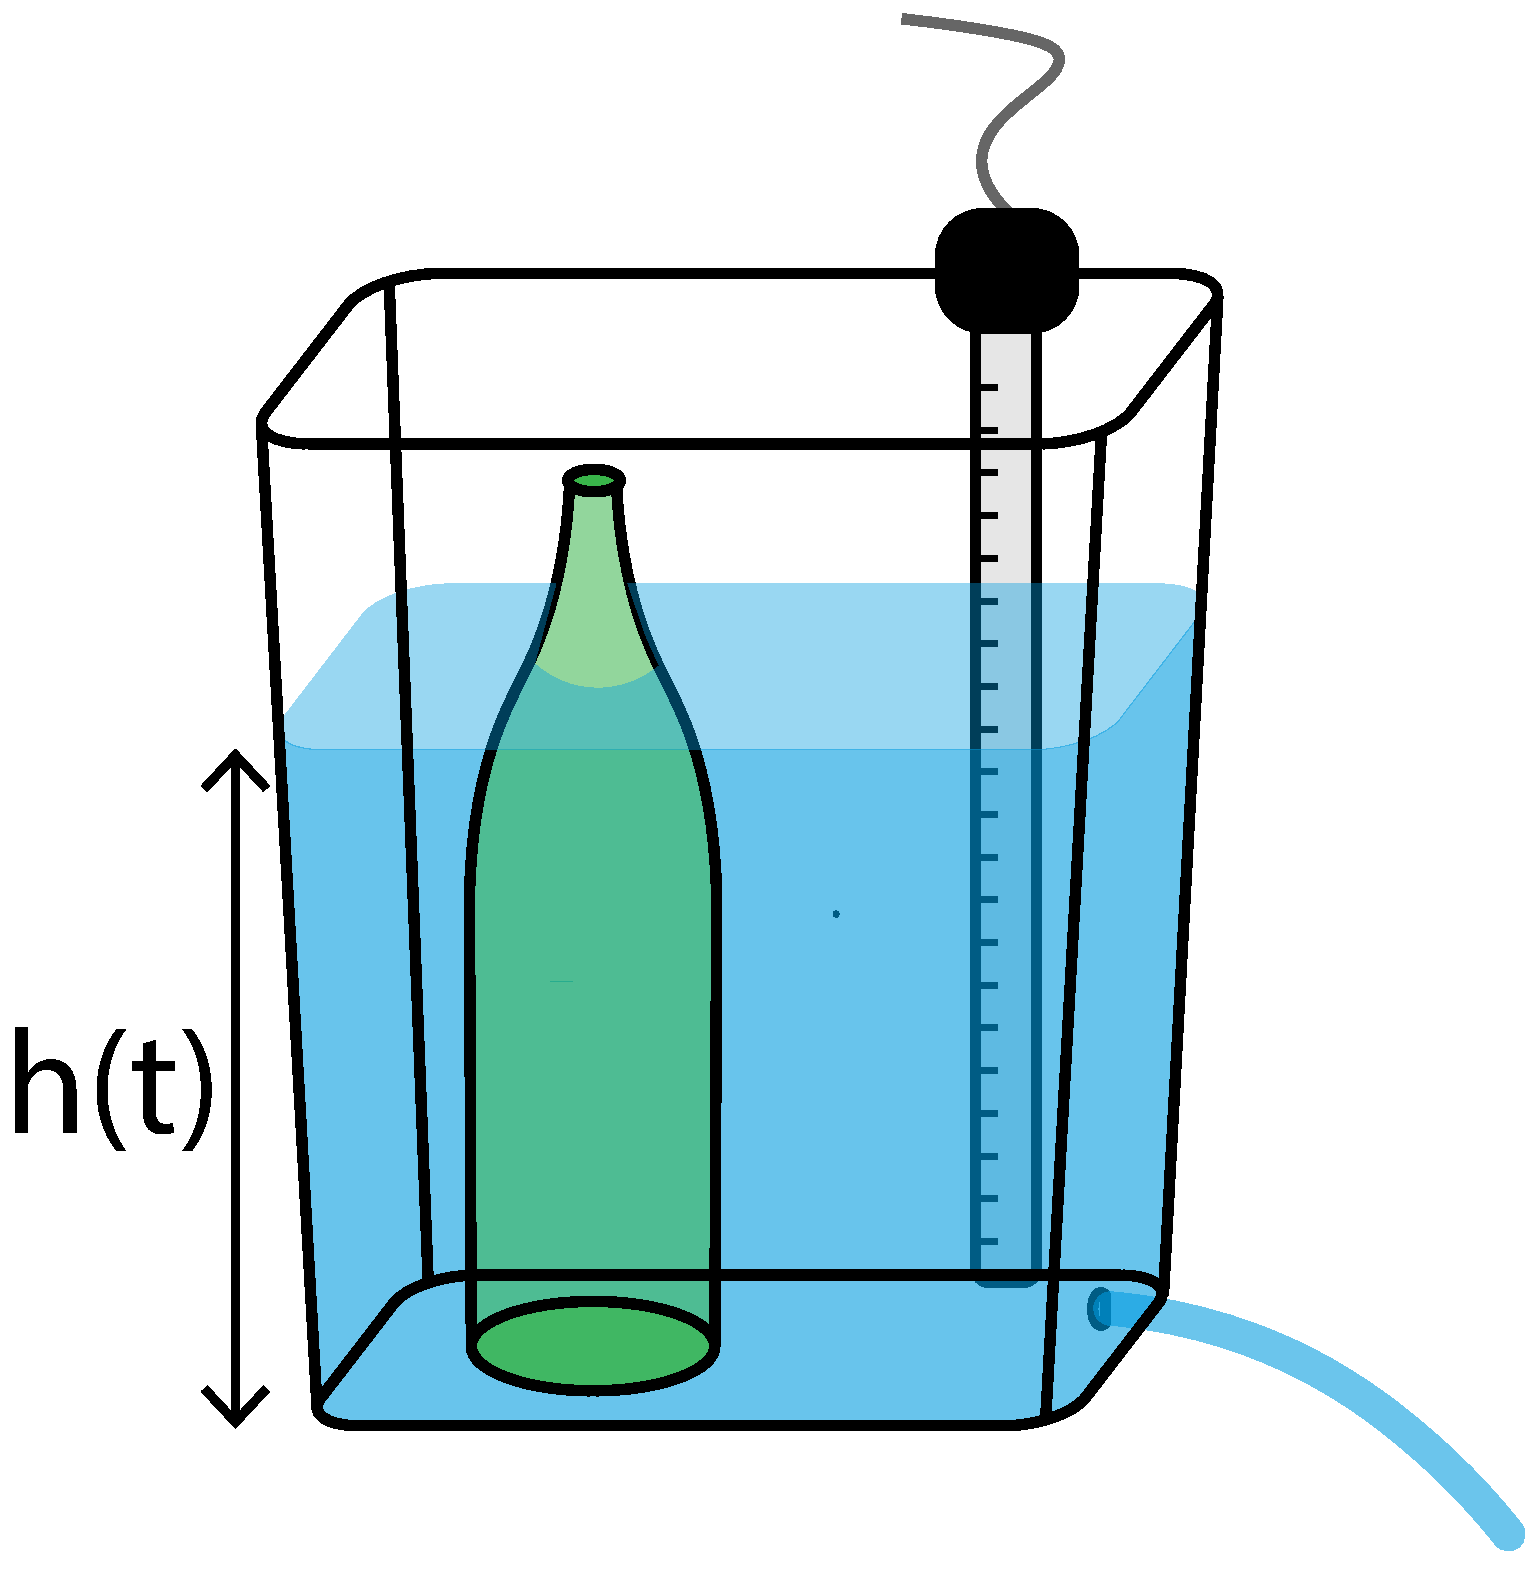
\includegraphics[height=0.375\textwidth]{../tank_geometry/tank_w_bottle.pdf}
	\includegraphics[height=0.375\textwidth]{../toy_h_w_object.pdf}
\end{center}

\absbreak % unclear why this is needed


\end{abstract}
%%%%%%%%%%%%%%%%%%%%%%%%%%%



\rsbreak

%%%%%%%%%% Insert the texts which can accomdate on firstpage in the tag "fmtext" %%%%%

\section{Introduction}
Throughout engineering and the applied sciences, we encounter a liquid-holding tank, draining via gravity-driven flow through a small orifice.
Mathematical models of the dynamics of the liquid level in a draining tank are useful for designing the geometry of the tank and orifice, predicting the emptying time, forecasting the outlet flow rate, controlling the liquid level by manipulating an input stream, and inferring the liquid level from the outlet flow rate \cite{d2021torricelli,seborg2016process,groetsch1993inverse,groetsch1999inverse}.

\begin{mytcbox}[label=box:waterclocks, breakable]{Ancient water clocks}
Interestingly, ancient societies (e.g. ancient Greece) exploited the empirically predictable dynamics of the water level in a draining container to measure and display the passage of time.
Specifically, the outflow \emph{clepsydra}, Greek for ``water thief'', was an open-top container with a small hole near its bottom and graduated markings on the inside. 
Filled with water then allowed to drain, the elapsed time was indicated by the liquid level with respect to the markings on the inside. \cite{bedini1962compartmented,hwang2021historical,ritner2016oriental,hejun1987research,schomberg2018karnak,mills1982newton}
The preserved Karnak clepsydra from $\sim$1300 BC \cite{schomberg2018karnak} is an inverted truncated cone. Notably, this geometry does not provide a constant rate of decrease in the water level; perhaps, though, its wider top was intended to compensate for faster outflow at higher water levels. An inverse problem pertaining to an outflow clepsydra is: what clepsydra shape provides a constant rate of decrease in the water level as it drains?
(Such a clepsydra may be obtained via a solid of revolution about the vertical axis such that the radius is proportional to the quartic root of the height. \cite{mills1982newton,d2021torricelli})
\end{mytcbox}
%Draining tanks have been studied since ancient times, as evidenced by water clocks in ancient Egypt, Greece, India, and China.
%The water clock, or clepsydra (Greek for ''water thief''), of the outflow design consisted of an open-top container, filled with water at some reference time, with a small orifice for outflow near its bottom.

%The geometry of an ideal clepsydra would produce a constant rate of decrease in the liquid level. However, the geometry of e.g. the preserved Karnak clepsydra from $\sim$1300 BC \cite{schomberg2018karnak}, an inverted truncated cone, does not. Though, perhaps, its wider top was intended to compensate for the faster outflow when the liquid level is higher.

% Italian physicist and mathematician 
Evangelista Torricelli (1608-1647) made a fundamental observation for mathematical modeling the liquid level in a tank draining via gravity-driven flow through a small orifice: the velocity $v$ at which liquid flows out of the orifice is proportional to the square root of the height of liquid above the orifice, $\Delta h$, i.e. $v\propto \sqrt{\Delta h}$ \cite{mills1982newton}.
% TODO: check that he didn't know g!
Today, we recover Torricelli's observation from Daniel Bernoulli's (1700–1782) equation \cite{welty2020fundamentals}, a mechanical energy balance applied to the steady, plug flow of an incompressible, inviscid fluid through the small orifice, neglecting frictional forces. This gives \emph{Torricelli's law}: $v=\sqrt{2 g \Delta h}$, with $g$ the acceleration due to gravity. \cite{d2021torricelli,teoman2022discharge}

Applying a mass balance and Torricelli's law to a tank draining of liquid via gravity-driven flow through a small orifice, we obtain a first-order, [generally] nonlinear differential equation governing the liquid level in the tank over time \cite{groetsch1993inverse,seborg2016process,debook}.
The geometry of the tank affects the dynamics of the liquid level through its cross-sectional area (parallel to the ground) as a function of height.
The cross-sectional area of the orifice affects the emptying time; theoretically, it gives the volumetric flow rate out of the tank from Torricelli's law. 
% TODO: a name for cross-sectional area parallel to the ground?
However, we must introduce a \emph{discharge coefficient} \cite{de2000pin,blasone2015discharge,wadhwa2021study,liu2008drainage} for the model to agree well with experimentally measured volumetric outflow rates \cite{farmer1992physical,driver1998torricelli,brady2009siphons,rother2024modelling,paldy1963apparatus,ivanov2014testing,williams2021vessel,pavesi2019investigating,planinvsivc2011holes,saleta2005experimental,lopac2015water,powell2012carrying}.
The discharge coefficient
(i) is defined as the ratio of the observed outlet volumetric flow rate to that predicted by Torricelli's law and the area of the orifice \cite{hicks2014determining};
(ii) accounts for the vena contracta of the liquid jet, frictional losses across the orifice, and non-uniformity of the velocity profile; and
(iii) depends on the rheology of the liquid, the geometry of the orifice, and, for laminar as opposed to turbulent flow, the Reynolds number \cite{teoman2022discharge}. 
The vena contracta refers to the lesser cross-sectional area of the liquid jet issuing from the orifice than the area of the orifice; this owes to fluid streamlines, inside the tank and near the orifice, not perpendicular to the orifice area \cite{horsch2020simple}. 
%  and (ii) depends on the rheology of the fluid and the geometry of the orifice. 
\cite{teoman2022discharge,hicks2014determining,blasone2015discharge,lienhard1984velocity,wadhwa2021study}

As opposed to the \emph{forward problem} of using a dynamic model to predict the trajectory of the liquid level in a draining tank, given the tank geometry, Groetsch \cite{groetsch1993inverse,groetsch1999inverse} posed an \emph{inverse problem} \cite{groetsch1993inverse,neto2012introduction,tarantola2005inverse}: reconstruct the shape of the tank from measurements of the liquid level over time as it drains. 
While impossible to infer the \emph{precise} geometry of the tank, determining the cross-sectional area of the tank as a function of height, from (a) the liquid level as a function of time and (b) the orifice area [and (c) the dynamic model of the liquid level], is a determined inverse problem. Although, this inverse problem is unstable: small errors in the measured liquid level can cause large errors in the estimated area of the tank. \cite{groetsch1993inverse}

\subsection{Our contribution}
Herein, we consider an inverse problem of reconstruction pertaining to a tank draining of liquid (due to gravity) through a small orifice in its side.
Suppose (i) we know the geometry of the tank and the orifice but (ii) the tank contains an exogenous heavy, solid object, whose shape is unknown.
To indirectly obtain information about the shape of the object, we fill the tank with liquid, then take measurements of the liquid level over time as the tank drains.
From this liquid level time series data, we wish
% and a differential equation model of the dynamics of the liquid level 
to infer the shape of the solid object inside the tank---particularly, its cross-sectional area as a function of height.

Explaining why this inverse problem is determined:
because the solid displaces liquid in the tank, the rate of change of the liquid level during draining indicates the cross-sectional area of the solid at the height of the liquid.
As the liquid level drops, the liquid ``scans'' the object's cross-sectional area as a function of its height. 

We conduct tank drainage experiments with water to collect liquid level time series data for illustrating and testing our ability to reconstruct the shape of an object inside the tank.
Because this reconstruction problem is unstable \cite{groetsch1993inverse}, we employ Bayesian statistical inversion \cite{calvetti2018inverse,waqar2023tutorial,kaipio2006statistical,dashti2013bayesian} to predict the object's area as a function of height \emph{with quantified uncertainty}.

%To demonstrate and test our ability to solve this reconstruction problem, we conduct tank drainage experiments to collect liquid level time series data.
%We drilled a small hole in the side of an open-top tank, near the bottom.
%For each experiment, we fill the tank (perhaps, containing an exogenous heavy, solid object) with water, then allow it to drain (driven by gravity). A liquid level sensor, communicating with an Arduino microcontroller, measures the liquid level over time, giving liquid level time series data. 


%In this Bayesian approach, we treat each parameter/input in the problem as a random variable and model its probability distribution.
%The prior distribution expresses our beliefs and information about the parameters/inputs \emph{before} liquid level time series data are collected.
%After a tank drainage experiment, we use (a) the [forward] dynamic model of the liquid level, (b) a probabilistic model of the noise in the measured liquid level, and (c) liquid level time series data to construct the likelihood function, which expresses the support the data lend for each possible parameter/input.
%Via Bayes's theorem, the posterior distribution of the parameters/inputs---conditioned upon the liquid level time series data---follows from the prior and likelihood. The posterior, the solution to the reconstruction problem, expresses a probability distribution over the object's cross-sectional area as a function of height, in light of the the liquid level time series data from a drainage experiment.

The structure of our paper is as follows. Sec.~\ref{sec:expt} describes our setup for tank drainage experiments.
In Sec.~\ref{sec:forward_model} we build (i) a forward model governing the dynamics of the liquid level in the tank given the tank, orifice, and object geometry and the discharge coefficient and (ii) a probabilistic model of the noise contaminating the measurements of the liquid level by our sensor.
Sec.~\ref{sec:bsi} gives a brief overview of Bayesian statistical inversion, a tool we employ to (1) calibrate our forward model then (2) solve the reconstruction problem.
In Sec.~\ref{sec:phaseI}, we calibrate (i.e., determine the posterior distribution of the parameters of) the forward and measurement models using length-measurements of the tank and orifice geometry and water level time series data from a drainage experiment concerning a tank \emph{lacking} an exogenous object. 
Finally, in Sec.~\ref{sec:phaseII}, we conduct a drainage experiment in a tank containing an exogenous object then leverage this water level time series data and our calibrated forward model to infer the area of the object in the tank as a function of height, with quantified uncertainty.
We test the posterior over the object's shape by comparing to our held-out measurement of it.

\section{Setup for tank drainage experiments} \label{sec:expt}
Here, we describe our experimental setup for tank drainage (of water) experiments.

We begin with a plastic, open-top tank with a small orifice drilled in its side, near the bottom and perpendicular to its face.
The tank is approximately an inverted, right, truncated cone whose base is a rounded rectangle. The cross-sectional area [parallel to the ground] of the tank as a function of height $h$ [cm] from its bottom base is:
\begin{equation}
	a(h) = \frac{h}{h_{\text{max}}}a_t + \left(1-\frac{h}{h_{\text{max}}}\right) a_b, \label{eq:a_of_h}
\end{equation}
with $h_{\text{max}}$ [cm] the height of the tank and $a_b$ [cm$^2$] and $a_t$ [cm$^2$] the area of the rounded rectangle forming the bottom and top, respectively, base of the tank.
The small, circular hole of radius $r_o$ [cm] in the side of the tank is a small height $h_o$ [cm] from the bottom base (to the hole's center).)

A tank draining experiment constitutes: (1) optionally, placing a heavy, solid object inside the tank; (2) filling the tank with water, to an initial height $h_0$ [cm]; (3) at time $t=0$ [s], allowing the water to drain out (driven by gravity) through the orifice; and (4) collecting time series data of the water level in the tank over time $\{(t_i, h_{\text{obs}, i}) \}$ using a liquid level sensor communicating with an Arduino microcontroller. See Fig.~\ref{fig:photo_of_tank}.

Note, the exogenous object (i) is heavier than water, thus remains at rest at the bottom of the tank throughout the process of draining and (ii) displaces water in the tank.
Let $\alpha(h)$ [cm$^2$] be the cross-sectional [parallel to the floor] area of this object as a function of height $h$.

\begin{figure}[h!]
\begin{center}
	\includegraphics[width=0.3\textwidth]{../tank_geometry/photo_of_tank.png}
	\caption{\textbf{Setup for tank drainage experiments.}
	We fill our open-top tank (perhaps, containing an exogenous object) with water, then allow it to drain via gravity-driven flow out of a small hole in its side, near its bottom. A liquid level strip measures the water level in the tank over time, giving time series data.
	}
	\label{fig:photo_of_tank}
\end{center}
\end{figure}

\paragraph{The liquid level sensor.}
We place our water level sensor, an eTape\texttrademark\xspace liquid level strip, vertically inside the tank, immersed in the water, to measure the water level in the tank at different times. The sensor communicates with an Arduino microcontroller, allowing us to automatically collect the time series data and write it to a file. 
The liquid level strip functions by virtue of being compressed by the hydrostatic pressure of the water in which it immersed; its resistive output is inversely proportional to the water level. 
\cite{eTape}
We constructed a calibration curve (a smooth 1D spline) with a resolution of 1 cm to map the reading from the level sensor [0-1023 integer values] to the liquid level in the tank [cm]. 

\section{The forward and measurement models and likelihood} \label{sec:forward_model}
The [deterministic] \emph{forward model} predicts the water level $h(t)$ [m] in our draining tank over time $t$ [s], given the \emph{inputs} $\alpha(h)$ and $h_0$ and \emph{parameters} $a_t$, $a_b$, $h_{\text{max}}$, $r_o$, $h_o$, the discharge coefficient $c$. 
The probabilistic \emph{measurement model} characterizes the noise contaminating a water level measurement $h_{\text{obs}}$ by our sensor.
After time series data \thedata are collected from a tank drainage experiment, the forward and measurement models give the \emph{likelihood function}: the probability density the data \thedata conditioned upon proposed functions/values for the inputs/parameters. 
When any of the inputs/parameters are uncertain, the likelihood function quantifies the support that the data \thedata lend for each possible set of inputs/parameters.

\subsection{Forward model}
Here, we mathematically model the height of water in our draining tank as a function of time, $h(t)$. (We assume the water at the top of the tank remains flat---allowed by a slow outflow rate). 
%We treat the water as incompressible (constant density: $\rho$ [g/cm$^3$]) and inviscid. 
%Our model follows from (i) the law of conservation of mass and (ii) Torricelli's law.
% outflow driven by gravity exerting a force on the water above the orifice, causing a hydrostatic pressure in the water at the entrance of the orifice. 


\paragraph{Torricelli's law.}
We model the velocity $v$ [cm/s] of the jet of water flowing out of the orifice at time $t$, when the water height is $h(t)$, with Torricelli's law \cite{d2021torricelli}:
\begin{equation}
	v(h(t)) =  \sqrt{2 g(h(t)-h_o)}, \label{eq:Torricelli}
\end{equation} where $g$ [cm/s$^2$] is the acceleration due to gravity. Torricelli's law follows from Bernoulli's equation \cite{welty2020fundamentals}, a mechanical energy balance on the flow through the orifice, treating (i) the flow as steady, plug, and absent of frictional forces and (ii) the water as inviscid and incompressible.
Torricelli's law matches (i) the gain in kinetic energy, $(\Delta m) v^2/2$, when a small mass $\Delta m$ of water is ejected from the orifice, with (ii) the loss of gravitational potential energy, $(\Delta m)g(h-h_o)$, from the concomitant removal of a small slice of water (of the same mass) from the top of the water in the tank. \cite{groetsch1993inverse,driver1998torricelli,williams2021vessel}

\paragraph{Volumetric outflow rate.}
%If Torricelli's law held and the cross-sectional area of the liquid jet out of the tank were the same as the cross-sectional area of the orifice ($\pi r_o^2$), the volumetric flow rate out of the tank would be $v\pi r_o^2$.
Invoking Torricelli's law, we model the volumetric flow rate out of the tank at time $t$, when the water height is $h(t)$, as:
\begin{equation}
	c \pi r_o^2 \sqrt{2 g(h(t)-h_o)}, \label{eq:outletflow}
\end{equation}
with $c\in(0,1)$ the [dimensionless] discharge coefficient---a ``fudge factor'' to account for the vena contracta in the water jet, non-plug flow through the orifice, and frictional losses as the water flows through the orifice \cite{horsch2020simple,teoman2022discharge,hicks2014determining,blasone2015discharge,lienhard1984velocity,wadhwa2021study}. 
Note, $c=1$ would imply a water jet whose cross-sectional area is equal to that of the orifice ($\pi r_o^2$), plug flow, and zero frictional losses.

\paragraph{Volume of water in the tank.} 
The volume $V$ [cm$^3$] of water in the tank at time $t$, when the water height is $h(t)$, follows from the method of cross-sections in calculus \cite{debook}:
\begin{equation}
	V(h(t))=\int_0^{h(t)} \left[a(y) - \alpha(y) \right] dy. \label{eq:volume}
\end{equation}
The integrand is the cross-sectional area of water in the tank at height $y$; subtraction of the area of the object $\alpha(y)$ from the area of the tank $a(h)$ in eqn.~\ref{eq:a_of_h} accounts for the displacement of water by the object in the tank. 
(We neglect the small volume of water displaced by the level sensor.)

\paragraph{Conservation of mass.}
Conservation of mass applied to the draining tank [as the control volume] at time $t \geq 0$ equates the rate of decrease of water in the tank [g/s] with the outflow rate [g/s]. Treating the water as incompressible (constant density: $\rho$ [g/cm$^3$]) and using the expression in eqn.~\ref{eq:outletflow} for the outflow rate, conservation of mass gives:
\begin{equation}
	\overbrace{\diff{}{t} \Bigl( \rho V(h(t)) \Bigr )}^{\text{rate of accumulation}}= - \overbrace{\rho c \pi r_o^2 \sqrt{2 g(h(t)-h_o)}}^{\text{outflow rate}}. \label{eq:massbalance}
\end{equation}
Differentiating $V(h(t))$ in eqn.~\ref{eq:volume} and using the chain rule \cite{debook} to rewrite the accumulation term gives our forward model for $h(t)$:
%\begin{empheq}[box=\mybox]{align}
\begin{empheq}[box={\Garybox[forward model]}]{align}
& \left[ a(h)-\alpha(h)\right] \diff{h}{t}= -c \pi r_o^2 \sqrt{2g (h(t)-h_o)}, \,\,\, t \geq 0 \label{eq:forward_model} \\
& h(0)=h_0, \nonumber
\end{empheq}
a [generally] nonlinear, first-order, ordinary differential equation (ODE) in $h(t)$ subject to an initial condition.
Given the tank and object geometry through $a(h)$ and $\alpha(h)$, the discharge coefficient $c$, the orifice radius and height $r_o$ and $h_o$, and initial water height $h_0$, we may numerically solve the ODE in eqn.~\ref{eq:forward_model} (we employ \texttt{DifferentialEquations.jl} \cite{rackauckas2017differentialequations}) to predict the water height in our draining tank over time, $h(t)$. 
% I.e., this \emph{forward} model makes predictions of the system output $h(t)$ (an \emph{effect}) when given the parameters and initial condition (the \emph{cause} of the effect).

\vspace{-\baselineskip}
\subparagraph{A regime of model invalidity.} If the radius of the orifice $r_o$ is small, surface tension may prevent water from flowing out of the orifice when $h- h_o$ is small yet positive. In this regime, Torricelli's law and thus our forward model do not hold.

\vspace{-\baselineskip}
\subparagraph{Parameterizing the object's area as a function of height.}
We parameterize the area of the object inside the tank as a function of height, $\alpha(h)$, with a list of $n+1$ discrete evaluations of $\alpha(h)$ on a uniform grid of points on its domain:
\begin{equation}
	\boldsymbol \alpha := [\alpha_0, \alpha_1, ... \alpha_n] \label{eq:alpha}
\end{equation}
where $\alpha_i :=\alpha(i \Delta h)$ for $i \in \{0, ..., n\}$, $\Delta h = h_{\text{max}}/n$. Then, we construct the function $\alpha(h)$ for $h\in [0, h_{\text{max}}]$ via linear interpolation of the function values in $\boldsymbol \alpha$. Equivalently, we represent the object's area as a function of height as:
\begin{equation}
	\alpha(h; \boldsymbol \alpha) = \sum_{i=0}^n \alpha_i \phi(h-i \Delta h) \label{eq:alpha_basis}
\end{equation} where $\phi(x)= \max(0, 1-\lvert x \rvert / (\Delta h)) $ is a triangle hat function \cite{hat_functions}.

\vspace{-\baselineskip}
\subparagraph{Inputs, output, and model parameters.} 
In the language of inverse problems \cite{groetsch1999inverse,waqar2023tutorial}, we refer to the object's area $\boldsymbol \alpha$ as an \emph{input} to the system (a \emph{cause}) and the water level as a function of time $h(t)$ as the \emph{output} of the system (an \emph{effect}).
The initial water level $h_0$ is also an input.  
The \emph{model parameters} $\boldsymbol \theta \in \mathbb{R}^6$ characterize the geometry of the tank and orifice and the rheology of water embedded in $c$:
\begin{equation}
	\boldsymbol \theta := [h_{\text{max}}, a_b, a_t, r_o, h_o, c]. \label{eq:theta}
\end{equation}
(We omit $g$ from $\boldsymbol \theta$ because we treat it as a constant known with certainty.)
Hereafter, we write the forward model as \themodel to indicate the dependence of $h(t)$ on the inputs and parameters.

\subsection{Measurement model}
Suppose at time $t$ our water level sensor measures the height of water in the tank, providing a data point $(t, h_{\text{obs}})$ (obs for ``observation''). 
To model [unobservable] noise corrupting the measurement, we treat the measured water level $h_{\text{obs}}$ as a realization of a random variable $H_{\text{obs}}$
\begin{equation}
	H_{\text{obs}} = \themodelnomath + \Psi,
\end{equation}
with the Gaussian-distributed random variable $\Psi \overset{\text{iid}}{\sim} \mathcal{N}(0, \sigma^2)$ representing the unobservable noise, additive to the model prediction \themodel and, among multiple measurements, independent and identically-distributed (iid). 
Then, the probability density governing the measured liquid level is a Gaussian with mean equal to the model prediction \themodel and variance $\sigma^2$:
\begin{equation}
	H_{\text{obs}} \mid h_0, \boldsymbol \alpha, \boldsymbol  \theta, \sigma^2 \sim \mathcal{N}(\themodelnomath, \sigma^2). \label{eq:H_obs_distn}
\end{equation} Here, we explicitly write that $H_{\text{obs}}$ is conditioned upon the initial water level, the object shape, the parameter vector, and the variance of the measurement noise.
% Sources of this noise are: imprecision of the liquid level strip, our calibration curve for the liquid level strip, vibrations

% TODO: plot residuals
% TODO expand 

\subsection{Likelihood function}
The likelihood is the $N$-dimensional probability density of observing time series data \thedata given the inputs $h_0$ and $\boldsymbol \alpha$, model parameters $\boldsymbol \theta$, and measurement noise variance $\sigma^2$. 
Based on eqn.~\ref{eq:H_obs_distn} and the iid assumption, the likelihood is:
\begin{equation}
 \pi_{\text{like}}(\thedatanomath \mid h_0,\boldsymbol  \alpha, \boldsymbol \theta, \sigma^2 ) = \prod_{i=1}^N \frac{1}{\sqrt{2\pi\sigma^2}} \exp \left[-\frac{1}{2}\left(\frac{h_{\text{obs}, i} - h(t_i; h_0, \boldsymbol\alpha, \boldsymbol\theta)}{\sigma} \right)^2 \right]. \label{eq:like}
\end{equation}
Once the data are obtained, the likelihood is viewed as a function of $h_0$, $\boldsymbol \alpha$, $\boldsymbol \theta$, and $\sigma^2$. The likelihood function scores the consistency between (i) the model predictions of the water level over time, with proposed values for the inputs and parameters, and (ii) the water level time series data. Hence, the likelihood function quantifies the support the data lend for each possible set of values for the inputs and parameters. 
% The key idea is: if the data were likely (unlikely) to be obtained under proposed values for the inputs and parameters, then the 

\section{Bayesian statistical inversion (BSI)} \label{sec:bsi}
Here, we briefly outline Bayesian statistical inversion (BSI)  \cite{calvetti2018inverse,waqar2023tutorial,kaipio2006statistical,dashti2013bayesian} as a tool to solve inverse problems associated with draining tanks while incorporating prior information and quantifying uncertainty in the solution. 
Later, we will employ BSI to, sequentially, (1, \emph{parameter inference}) calibrate our forward and measurement models using length-measurements of the tank and orifice and tank drainage time series data collected when the tank certainly does not contain a solid object then (2, \emph{reconstruction}) infer the shape of an unknown object inside of the tank using the calibrated model and tank drainage time series data collected when an object resides in the tank.

For inverse problems associated with draining tanks, we treat the uncertain input(s) and/or parameters as random variables and model their probability distributions. 
The region(s) of input/parameter space containing most of the density represent our knowledge and beliefs about where the input/parameters most likely lie. And, the degree of spread of the density reflects our uncertainty. We may succinctly summarize the state of our knowledge and beliefs about an input/parameter through the moments of its probability distribution (e.g., mean and variance) with the other inputs/parameters marginalized out. 

BSI proceeds in three stages:

\vspace{-\baselineskip}
\paragraph{(1) specify a prior probability distribution.}
First, we specify a \emph{prior} probability density $\pi_{\text{pr}}(h_0, \boldsymbol \alpha, \boldsymbol \theta, \sigma^2)$ expressing our knowledge and beliefs about the initial water level $h_0$, object shape $\boldsymbol \alpha$, parameter vector $\boldsymbol \theta$, and measurement noise variance $\sigma^2$ \emph{before} we allow the tank to drain and collect water level time series data.
The prior density we impose on an input/parameter can range from (i) diffuse (e.g. a uniform distribution) if we have no knowledge about it, adopting the principle of indifference, to (ii) informative (e.g. a Gaussian with a small variance) if we made a [noisy] measurement of it. Regardless, prior distributions contain some degree of subjectivity.
\cite{van2021bayesian}

\vspace{-\baselineskip}
\paragraph{(2) conduct an experiment to collect data.}
Next, we conduct a tank-drainage experiment (containing a solid object, or not) to collect water level time series data, \thedata. 
When this data are considered against the forward and measurement models, the data provide new information about the inputs and parameters. 
That is, compared to the prior distribution, the data may lend more support for some values of the inputs/parameters and contradict other values.

\vspace{-\baselineskip}
\paragraph{(3) update the prior to a posterior probability distribution.}
In light of the data \thedata we collected, we update the prior distribution of the inputs and parameters to a \emph{posterior} probability density $\pi_{\text{post}}(h_0, \boldsymbol \alpha, \boldsymbol \theta, \sigma^2 \mid \thedatanomath)$. I.e., we are conditioning the inputs and parameters upon the data.
The posterior density follows from the likelihood function in eqn.~\ref{eq:like} and prior density via Bayes's theorem \cite{van2021bayesian,calvetti2018inverse}:
\begin{equation}
	\pi_{\text{post}}(h_0, \boldsymbol \alpha, \boldsymbol \theta, \sigma^2 \mid \thedatanomath) = \frac{
	\pi_{\text{like}}(\thedatanomath \mid h_0,  \boldsymbol \alpha, \boldsymbol \theta, \sigma^2 ) 
	\pi_{\text{pr}}(h_0, \boldsymbol\alpha, \boldsymbol \theta, \sigma^2)
	}{
	\pi_{\text{ev}}(\thedatanomath) 
	}, \label{eq:post}
\end{equation} where the denominator, the \emph{evidence}, is the marginal likelihood:
\begin{multline}
    \pi_{\text{ev}}(\thedatanomath) = \\ 
    \int_0^\infty
     \int_{\mathbb{R}^6}  
     \int_{\mathbb{R}^{n+1}} 
     \int_0^\infty 
    \pi_{\text{like}}(\thedatanomath \mid h_0,  \boldsymbol \alpha, \boldsymbol \theta, \sigma^2 ) 
	\pi_{\text{pr}}(h_0, \boldsymbol\alpha, \boldsymbol \theta, \sigma^2)
	dh_0 d \boldsymbol\alpha d \boldsymbol\theta d\sigma^2 \label{eq:ev}
\end{multline}
that can in principle be computed from the likelihood and prior in the numerator. 

The posterior represents the raw, uncertainty-quantifying solution to the inverse problem: it expresses the state of our knowledge and beliefs about the inputs and parameters in light of the experimental tank drainage data, when compared with the forward and measurement models. 
The posterior assigns a weight to each possible value of the inputs/parameters $h_0, \boldsymbol \alpha, \boldsymbol \theta, \sigma^2$ that could explain the data \cite{dashti2013bayesian}. 
% Assuming the forward and measurement models and prior assumptions hold, the inputs/parameters plausibly belong to the region of input/parameter space containing the bulk of the posterior density, and the spread (concentration) of the posterior over this space quantifies our uncertainty (certainty) about the inputs/parameters.
% We may summarize the posterior distribution of an input/parameter with a \emph{credible interval} that contains the bulk of the posterior density. 
% E.g., the 95\% equal-tailed credible interval for a variable contains 95\% of the posterior density with equal-area tails omitted on both sides.
The posterior may be 
(i) summarized with a \emph{credible region} [that contains the bulk of the posterior density] for each parameter/input;
(ii) queried e.g., ``what is the probability this input/parameter exceeds a certain value?''; and
(iii) exploited in conjunction with the forward model to make probabilistic predictions, such as predicting the distribution of emptying times for a draining tank.

\vspace{-\baselineskip}
\subparagraph{Sampling from the posterior distribution.} We resort to Markov chain Monte Carlo (MCMC) simulations \cite{robert1999monte} to obtain [serially-correlated, sequential] samples \thesamples from the posterior density $\pi_{\text{post}}(h_0, \boldsymbol \alpha, \boldsymbol \theta, \sigma^2 \mid \thedatanomath)$. 
Advantageously, MCMC samplers allow us to circumvent computing the evidence $\pi_{\text{ev}}(\thedatanomath)$ in eqn.~\ref{eq:ev}, a high-dimensional integral.  From the samples \thesamples from the posterior distribution, we may draw empirical posterior distributions (histograms), compute credible intervals, and plot samples of liquid level trajectories when paired with the forward model.
Specifically, we employ the No-U-Turn Sampler (NUTS) \cite{hoffman2014no} implemented in the probabilistic programming language \cite{gordon2014probabilistic} \texttt{Turing.jl} \cite{ge2018turing}.

\section{Results}
We now employ BSI to:
(1) calibrate our forward and measurement models, then
(2) exploit our calibrated model to infer the shape of a solid, heavy object using water level time series data from a tank drainage experiment with that object inside of the tank.

\subsection{Phase I: Bayesian calibration of the forward and measurement models}
\label{sec:phaseI}
In Phase I, our objective is to calibrate then test our forward and measurement models in eqn.~\ref{eq:forward_model} and \ref{eq:H_obs_distn}.
For calibration, we (a) make length-measurements of our tank and orifice geometry and (b) collect water level time series data from a tank drainage experiment certainly \emph{without} an object inside the tank (so, $\boldsymbol \alpha = \mathbf{0}$ with certainty).
These data provide information about the model parameters $\boldsymbol \Theta$ and measurement noise variance $\Sigma^2$. 
The main product of ``Phase I: model calibration'' is the posterior distribution of $\boldsymbol \Theta$ and $\Sigma^2$.
The forward and measurement models paired with this posterior distribution constitute the \emph{calibrated model}. 
% The key idea is that our length-measurements of the tank and orifice geometry and water level time series data from a drainage experiment in a tank without an object provide information about the parameters and measurement noise variance. 
Hopefully, the calibrated model will allow us to accuracy solve the reconstruction problem in Phase II. 
% Here, we also conduct a replicate experiment for testing the calibrated model. 
% Since we directly measured the other parameters in $\theta$, the two primary unknowns for our model calibration phase are the discharge coefficient $C$ and noise variance $\Sigma^2$. 

\subsubsection{Experimental setup}
We set up a tank draining experiment (see Sec.~\ref{sec:expt}) with an initial water level (measured by the level strip) $h_{0, \text{obs}}=26.54$\,cm. 
With certainty, no heavy, solid object resides in the tank. 
See Fig.~\ref{fig:naked_tank}.

\subsubsection{Prior distributions} 
Below, we express our knowledge and beliefs about the inputs and parameters, before allowing the tank to train and collecting water level time series data, by constructing a prior probability density $\pi_{\text{pr}}(h_0, \boldsymbol \alpha, \boldsymbol \theta, \sigma^2)$. (In our prior distribution, most variables are independent of the others; hence, we specify the prior density variable-by-variable.)

\vspace{-\baselineskip}
\subparagraph{Tank geometry.} We employ a measuring tape to make length-measurements of the dimensions of the tank.
Based on these measurements, our estimates for the area of the rounded rectangle forming the top and bottom of the tank are $a_{t, \text{obs}}=129.9$\,cm and $a_{b, \text{obs}}=103.0$\,cm. Our measured tank height is $h_{\text{max, obs}}=28.6$\,cm.
The following prior distributions, informed by our [admittedly, noisy and imprecise] measurements, reflect our knowledge and beliefs about the tank geometry (see eqn.~\ref{eq:a_of_h}):
\begin{align}
A_t &\sim \mathcal{N}(a_{t, \text{obs}}, \sigma_\ell^2/2) \label{eq:A_t_prior} \\
A_b &\sim \mathcal{N}(a_{b, \text{obs}}, \sigma_\ell^2/2) \\
H_{\text{max}} &\sim \mathcal{N}(h_{\text{max}, \text{obs}}, \sigma_\ell^2)
\end{align}
where $\sigma_\ell=0.1$\,cm is our assumed standard deviation of our length-measurements, based on the distance between markings on our measurement tape. 
(The factor of $1/2$ in the variance for $A_t$ and $A_b$ arises from the variance of a product of Gaussian random variables \cite{bromiley2003products}.)

\vspace{-\baselineskip}
\subparagraph{Orifice height and geometry.} 
We measure the height of the orifice in the side of the tank as $h_{o, \text{obs}}=0.9$\,cm and impose an informative prior:
\begin{equation}
H_o \sim \mathcal{N}(h_{o, \text{obs}}, \sigma_\ell^2).
\end{equation}
Informed by the manufacturer-reported diameter (5/64\,in) of the drill bit we used to drill the hole in the tank, we estimate the radius of the orifice as $r_{o, \text{obs}}=0.1$\,cm and impose the prior:
\begin{equation}
R_o \sim \mathcal{N}(r_{o, \text{obs}}, \sigma_d^2), \label{eq:R_o_prior}
\end{equation}
where $\sigma_d= 0.001$\,cm accounts for uncertainty in the drill bit radius and its translation into an orifice radius.

\vspace{-\baselineskip}
\subparagraph{Exogenous object geometry.}
With certainty, no solid object resides in the tank, so $\boldsymbol \alpha=\mathbf{0}$ with certainty. Technically, this is a Dirac delta prior density on $\mathbf{A}$, $\pi_{\text{pr}}(\boldsymbol \alpha)=\delta(\boldsymbol \alpha - \mathbf{0})$. 


% TODO mention truncations


\vspace{-\baselineskip}
\subparagraph{Discharge coefficient.} 
We impose a weakly informative prior distribution on the discharge coefficient
\begin{equation}
	C \sim \mathcal{N}(0.65, 0.25^2),
\end{equation} whose mean is informed by a reported discharge coefficient for water flow through a round orifice \cite{hicks2014determining}. 

\vspace{-\baselineskip}
\subparagraph{Variance of measurement noise.} 
We impose a uniform prior on the standard deviation of the noise emanating from our water level sensor:
\begin{equation}
\Sigma \sim \mathcal{U}(0\,\text{cm}, 0.5\,\text{cm}),
\end{equation} whose generous upper bound is informed by our experience in calibrating the liquid level strip. 

\vspace{-\baselineskip}
\subparagraph{Initial water level.} We impose an informative prior distribution on the initial water level based on the initial reading of the water level sensor:
\begin{equation}
	H_0 \mid \Sigma=\sigma \sim \mathcal{N}(h_{0, \text{obs}}, \sigma^2),
\end{equation} where $\sigma^2$ is the variance of the noise from the level sensor in our measurement model.

\paragraph{Visualization of the prior.}
Together with the forward model in eqn.~\ref{eq:forward_model}, $\pi_{\text{pr}}(h_0, \boldsymbol \alpha, \boldsymbol \theta, \sigma^2)$ gives a prior distribution over water level trajectories in the tank, \themodel. 
To visualize and interpret the prior, Fig~\ref{fig:prior_train} shows samples of functions \themodel from the prior. The prior encodes a broad range of possible future water level trajectories. 

\subsubsection{Water level time series data from a tank-drainage experiment} At time $t:=0$, we allow our tank to drain of water through the small orifice in its side. Our liquid level sensor records the water level in the tank over time. The resulting water level time series data \thedata are shown in Fig.~\ref{fig:posterior_train}.

\subsubsection{Posterior distribution}
Given our prior probability density $\pi_{\text{pr}}(h_0, \boldsymbol \alpha, \boldsymbol \theta, \sigma^2)$ and data \thedata from which we construct the likelihood function in eqn.~\ref{eq:like}, the posterior distribution $\pi_{\text{post}}(h_0, \boldsymbol \alpha, \boldsymbol \theta, \sigma^2 \mid \thedatanomath)$ follows from Bayes's theorem in eqn.~\ref{eq:post}. 
We employ the MCMC sampler, NUTS, to obtain samples \thesamples from the posterior distribution. 

%TODO how many samples

\paragraph{Visualization of the posterior.}Fig.~\ref{fig:posterior_train_theta} visualizes the posterior distribution. 
The top panel shows the [marginal] empirical posterior distributions (histograms) of the parameters and initial water level along with their 80\% equal-tailed credible intervals. 
For the variables we measured with our measuring tape, the credible interval is centered at the measurement. 
The measured initial water level, however, falls outside of the credible interval; a higher initial water level than measured is consistent with the time series data \thedata.
The bottom panel shows the covariance matrix of the parameters and inputs. 

%The information that the data from this tank-draining experiment provided about $C$ and $\Sigma$ will be useful for the reconstruction inverse problem of inferring the shape of an object inside the tank from water level time series data. (We assume the object does not affect the discharge coefficient nor noise in the liquid level sensor.)

\paragraph{Posterior predictive check.} We plot water level trajectories \themodel with $(\thevars)$ sampled from the posterior distribution, in Fig.~\ref{fig:posterior_train}. 
The posterior models reasonably agree with the measured water levels over time (mean absolute residual: 0.26\,cm). 
Comparing the water level trajectories sampled from the posterior in Fig.~\ref{fig:posterior_train} with those from the prior Fig.~\ref{fig:prior_train}, the much lower variance in the posterior indicate the large amount of information the water level time series data provided about the parameter vector.

\begin{figure}[!ht]
    \centering
        \begin{subfigure}[b]{0.22\textwidth}
    	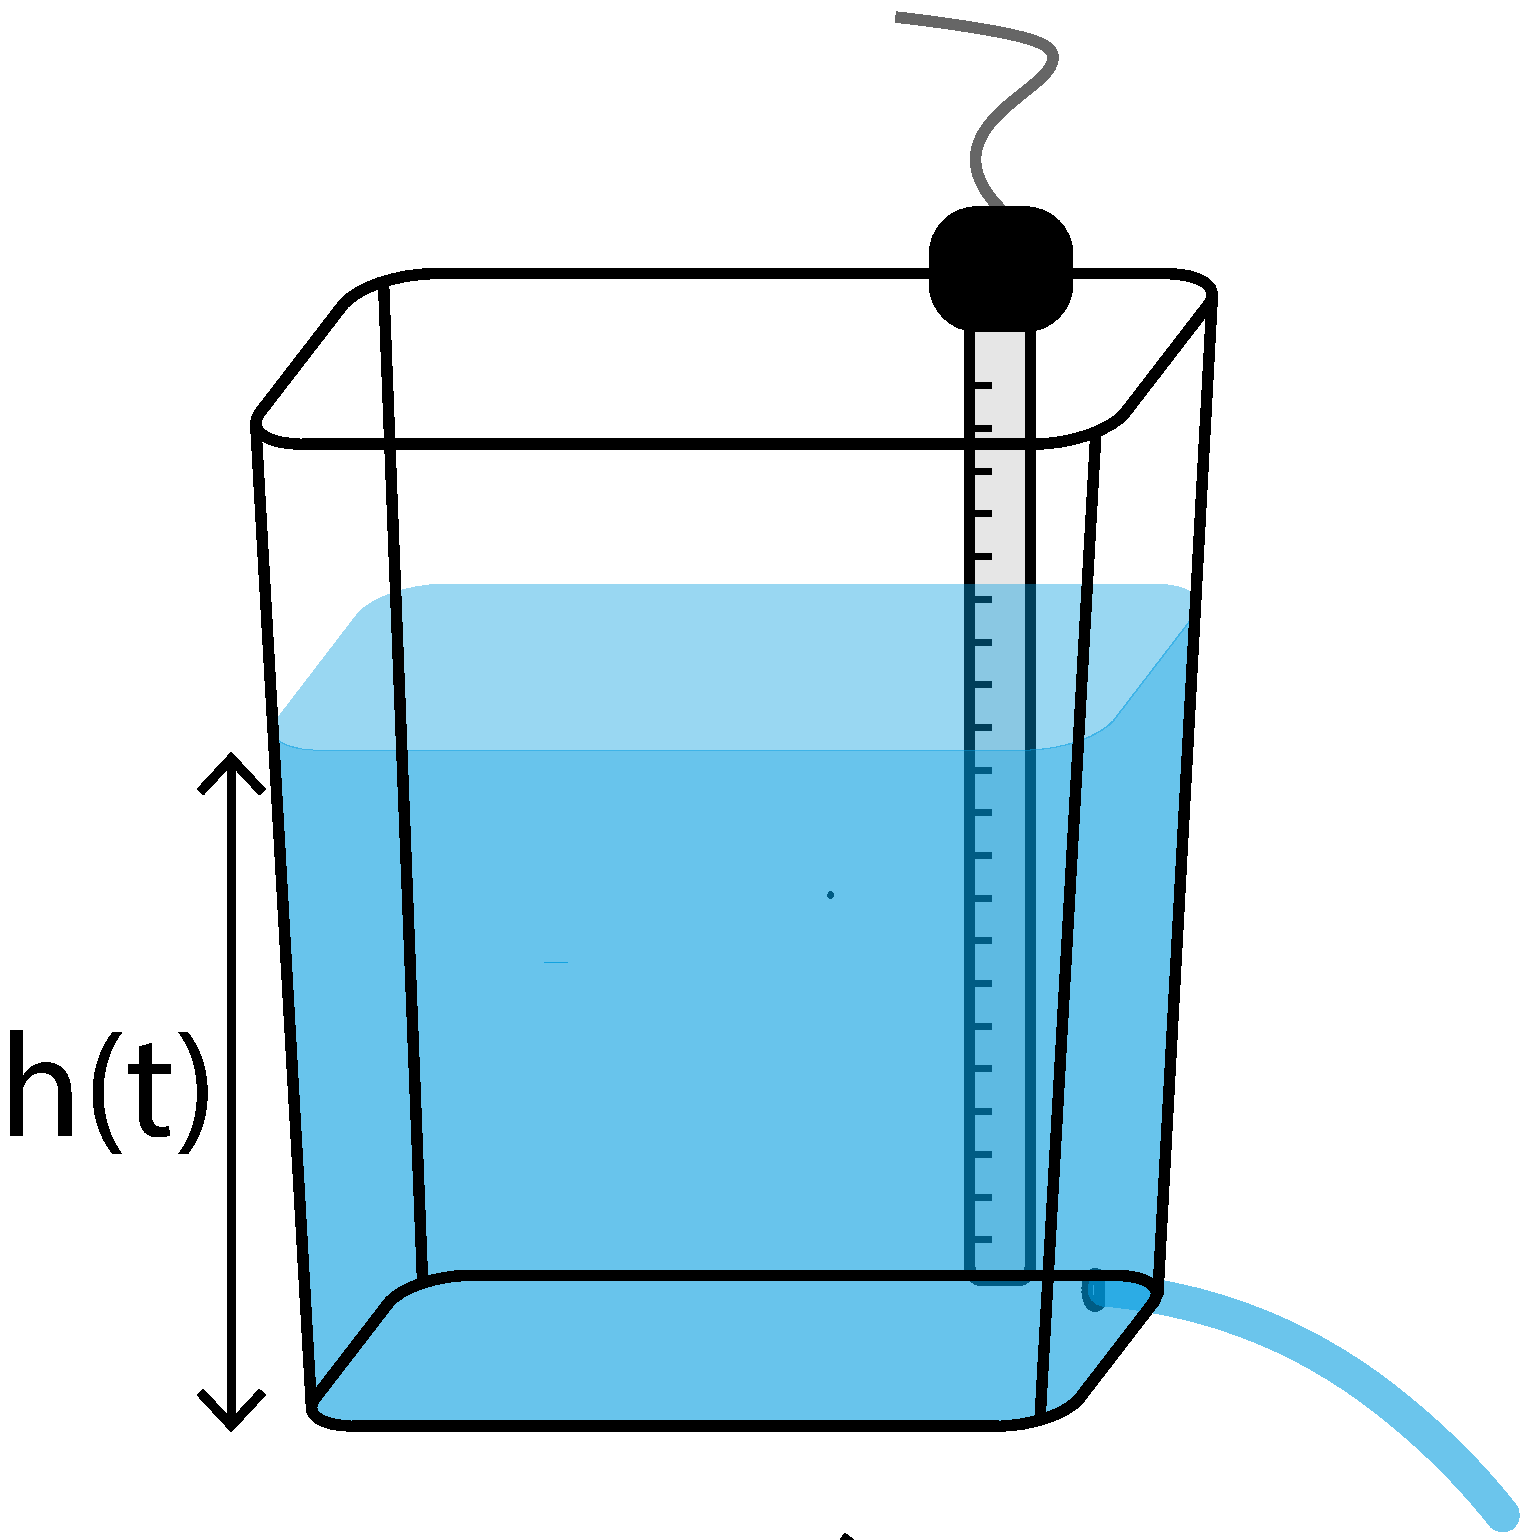
\includegraphics[width=\textwidth]{../tank_geometry/naked_tank.pdf}
	\caption{Experiment setup} \label{fig:naked_tank}
    \end{subfigure}
    
     \begin{subfigure}[b]{0.4\textwidth}
    	\includegraphics[width=\textwidth]{../prior_train.pdf}
	\caption{Prior distribution} \label{fig:prior_train}
    \end{subfigure}
     \begin{subfigure}[b]{0.4\textwidth}
    	\includegraphics[width=\textwidth]{../posterior_train.pdf}
	\caption{Data \& posterior distribution} \label{fig:posterior_train}
    \end{subfigure}
    
     \begin{subfigure}[b]{\textwidth}
     \center
    	\includegraphics[width=0.72\textwidth]{../posterior_train_theta.pdf}
	\includegraphics[width=0.34\textwidth]{../posterior_cov_matrix.pdf}
	\caption{Posterior distribution} \label{fig:posterior_train_theta}
    \end{subfigure}
    \caption{
      \textbf{Model calibration.}
      (a) We fill our empty tank with water, then, at $t=0$, allow it to drain through the orifice in its side.
      (b) Samples of water level trajectories \themodel from the prior probability density $\pi_{\text{pr}}(\thevars)$.
      (c) Time series data \thedata from the tank drainage experiment and samples of water level trajectories \themodel from the posterior distribution $\pi_{\text{post}}(\thevars \mid \thedatanomath)$.
      (d) Visualizing the posterior distribution $\pi_{\text{post}}(\thevars \mid \thedatanomath)$. Top: marginals. Bottom: covariance matrix.      
      }
\end{figure}

\paragraph{The calibrated model.} The forward and measurement models in eqn.~\ref{eq:forward_model} and \ref{eq:H_obs_distn} together with the posterior distribution $\pi_{\text{post}}(\boldsymbol \theta, \boldsymbol \sigma^2 \mid \thedatanomath)$ (with $h_0$ marginalized out and $\boldsymbol \alpha=\mathbf{0}$) constitute the \emph{calibrated model}.
 The calibrated model will be useful for solving the reconstruction problem in phase II, because the presence of an object inside the tank presumably does not affect the parameter vector $\boldsymbol \theta$ nor the measurement noise variance $\sigma^2$ of the level sensor.
We approximate the posterior distribution as a multi-variate Gaussian distribution
\begin{equation}
	\begin{bmatrix} \boldsymbol \Theta \\ \Sigma \end{bmatrix} \mid \thedatanomath \sim \mathcal{N}(\mathbf{m}, \mathbf{C}) \label{eq:post_theta_sigma}
\end{equation}
with mean $\mathbf{m}$ and covariance matrix $\mathbf{C}$ computed from our MCMC samples $(\boldsymbol \theta_i, \sigma_i)_{i=1}^{N_s}$ from the posterior. 
(The means of each parameter in $\mathbf{m}$ and the covariance matrix $\mathbf{C}$ are displayed in Fig.~\ref{fig:posterior_train_theta}.)

\subsubsection{A replicate experiment for testing the calibrated model}
We now test our calibrated model for its ability to predict the dynamics of the water level in our tank in a new, replicate drainage experiment (also without an object inside, so $\boldsymbol \alpha=\mathbf{0}$) with measured initial water level $h_{0, \text{obs}}=26.49$\,cm. 
We sample water level trajectories \themodel predicted by the calibrated model by (1) sampling a $\boldsymbol \theta$ and $\sigma$ from the empirical posterior distribution, (2) sampling an initial water level from $H_0 \mid \Sigma=\sigma \sim \mathcal{N}(h_{0, \text{obs}}, \sigma^2)$, then (3) numerically solving the forward model to obtain \themodel.
Fig.~\ref{fig:test} compares the water level time series data collected from the replicate experiment, \thedata, with the trajectories \themodel predicted by the calibrated model. We observe good agreement between the predictions by the calibrated model and the experimental data (mean absolute residual: 0.28\,cm). For kicks, we also show the distribution of predicted tank-emptying times.

\begin{figure}[h!]
    \centering
    	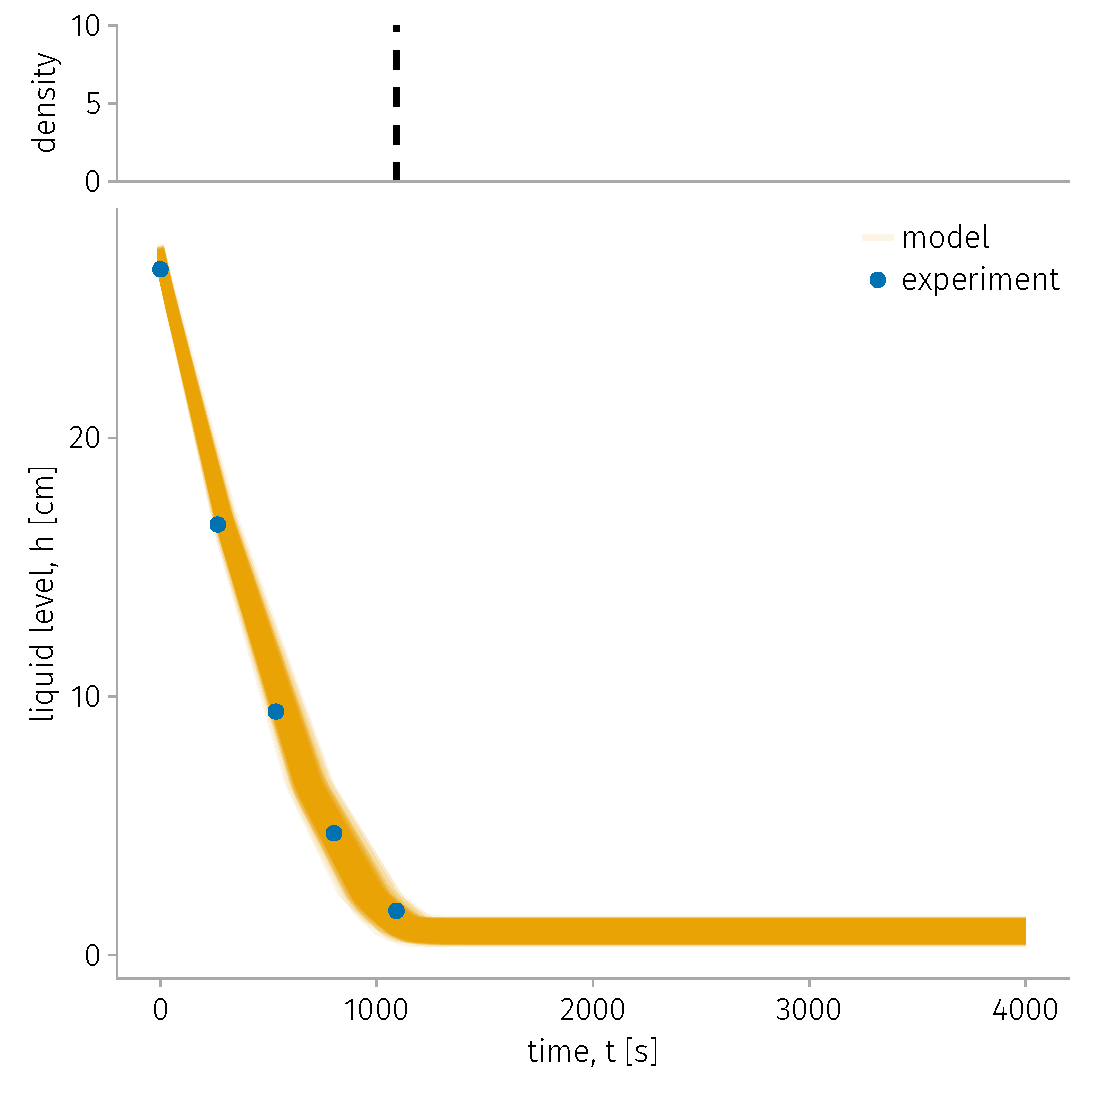
\includegraphics[width=0.5\textwidth]{../test.pdf}
    \caption{
      \textbf{Testing the calibrated forward model.}
      In a replicate tank-draining experiment without an object, we show (top) the predicted distribution of emptying times and (bottom) the water level time series data together with samples of the water level trajectory predicted by the calibrated forward model. Note, besides the measured initial water level, the time series data was held out from the model predictions and thus serves as test data.
      } \label{fig:test}
\end{figure}

\subsection{Phase II: Bayesian inference of the shape of an object inside the tank} \label{sec:phaseII}
Finally, we exploit our calibrated model to infer the shape of a heavy, solid object placed inside of our tank, using water level time series data as the tank containing this object drains.
Our objective is to obtain the posterior distribution of $\mathbf{A}$ that characterizes the cross-sectional area of the object as a function of height, $\alpha(h)$ (see eqn.~\ref{eq:alpha}).
This constitutes a reconstruction inverse problem---we aim to reconstruct an input from the observed output.

\subsection{Experimental setup}
We set up a tank draining experiment (see Sec.~\ref{sec:expt}) by:
(i) placing a heavy, solid object inside of the tank, which remains stationary---a large glass bottle;
(ii) fill the tank to an initial water level (measured by the level strip) of $h_{0, \text{obs}}=26.49$\,cm. 
See Fig.~\ref{fig:tank_w_bottle}.


\subsection{Prior distributions}
%Our prior distribution for (i) the initial water level $H_0$ is informed by the initial water level measurement; (ii) the parameter vector $\boldsymbol \Theta$ and measurement noise variance $\Sigma^2$ is informed by the model calibration phase; and (iii) the object area $\mathbf{A}$ (a) is diffuse, to entertain a large range of possible object shapes in the tank, and (b) promotes a smooth function $\alpha(h)$. Fig.~\ref{fig:prior_area} displays samples from the prior distribution for the object shape vector $\mathbf{A}$. 
% Below, we express our knowledge and beliefs about the inputs and parameters, before allowing the tank to train and collecting water level time series data, by constructing a prior probability density $\pi_{\text{pr}}(h_0, \boldsymbol \alpha, \boldsymbol \theta, \sigma^2)$. 

% \vspace{-\baselineskip}
\subparagraph{The parameter vector and measurement noise variance.}
Abiding by the adage ``yesterday's posterior is today's prior'' \cite{calvetti2010subjective}, 
our posterior distribution of the model parameter vector $\boldsymbol \Theta$ and measurement noise variance $\Sigma^2$ from ``Phase I: model calibration'', the multi-variate Gaussian in eqn.~\ref{eq:post_theta_sigma}, becomes our prior distribution for this reconstruction problem in Phase II.
This constitutes exploitation of our calibrated model from Phase I.
(An underlying, highly-plausible assumption is that the object inside the tank does not affect the discharge coefficient.)

\vspace{-\baselineskip}
\subparagraph{Initial water level.} We impose an informative prior distribution on the initial water level based on the initial reading of the water level sensor:
\begin{equation}
	H_0 \mid \Sigma = \sigma \sim \mathcal{N}(h_{0, \text{obs}}, \sigma^2),
\end{equation} where $\sigma^2$ is the variance of the noise from the level sensor in our measurement model.

\vspace{-\baselineskip}
\subparagraph{Shape of the object.}
Our prior beliefs about the shape of the object in the tank are:
(i) regarding the area of its bottom base, we adopt the principle of indifference and equally entertain possibilities ranging from the absence of an object to the presence of the largest object that can sink to the bottom of the tank;
and
(ii) the cross-sectional area of the object as a function of height, $\alpha(h)$, is a relatively smooth function.
The latter aims to counter the unstable nature of this inverse problem \cite{groetsch1993inverse}.

Specifically, we impose a uniform distribution on the cross-sectional area of the object at $h=0$, $A_0$ (the random variable representing $\alpha(0)$):
\begin{equation}
	A_0 \mid A_b=a_b \sim \mathcal{U}(0, a_b).
\end{equation}
That is, the area of the bottom base of the object could range from zero (no object) to that of the bottom of the tank (largest that can fit in the tank), $a_b$. By adopting the principe of indifference and imposing this diffuse prior, we will allow the water level time series data to ``speak for itself'' about the shape of the object in the tank.

For the smoothness prior \cite{calvetti2018inverse}, we sequentially correlate the remainder of the random variables characterizing the object's area, $A_1, ..., A_n$: 
\begin{equation}
 A_i - A_{i-1} \sim \mathcal{N}(0, \gamma^2) \text{ for } i \in \{1, ..., n\}.
\end{equation} 
The zero mean Gaussian distribution on the difference in the area of the object at two adjacent heights means we expect the function $\alpha(h)$ to be flat and change slowly. 
The variance hyperparameter $\gamma^2$ controls the degree to which we promote smoothness in our representation of $\alpha(h)$ by $\mathbf{A}$. Specifically, a smaller $\gamma^2$ promotes a smaller difference between adjacent areas and thus a more smooth $\alpha(h)$. 

\paragraph{Visualization of the prior.}
Fig.~\ref{fig:prior_area} displays samples of $\mathbf{A}$ from the prior distribution, each of which translates into a realization of the object's area as a function of height $\alpha(h)$. This is a visualization of our beliefs about the shape of the object in the tank before water level time series data from the ``object scan'' are collected and considered against the forward model.

\subsection{Water level time series data from a tank-drainage experiment}
At time $t:=0$, we allow our tank to drain of water through the orifice in its side. The liquid level sensor records the water level in the tank over time, giving the data \thedata in Fig.~\ref{fig:posterior_object}.

\subsection{Posterior distribution}
%Via Bayes's theorem in , the posterior distribution $\pi_{\text{post}}(h_0, \boldsymbol \alpha, \boldsymbol \theta, \sigma^2 \mid \thedatanomath)$ follows from (i) prior probability density $\pi_{\text{pr}}(h_0, \boldsymbol \alpha, \boldsymbol \theta, \sigma^2)$---informed for $H_0$, $\boldsymbol \Theta$, and $\Sigma^2$ and diffuse but smooth for $\mathbf{A}$---and (ii) tank drainage data \thedata, from which we construct the likelihood function in eqn.~\ref{eq:like}, the posterior distribution $\pi_{\text{post}}(h_0, \boldsymbol \alpha, \boldsymbol \theta, \sigma^2 \mid \thedatanomath)$ follows from Bayes's theorem in eqn.~\ref{eq:post}. 
%We employ the MCMC sampler, NUTS, to obtain samples $\{(h_{0,i}, \boldsymbol \alpha_i, \boldsymbol \theta_i, \sigma^2_i\}$ from the posterior distribution. 



\paragraph{Visualization of the posterior.} Fig.~\ref{fig:posterior_area} shows the solution to the reconstruction problem: samples of the inferred area of the object as a function of height, constructed from $\boldsymbol \alpha$ sampled from the posterior distribution. 
For comparison, our measurements of the object's area at different heights---held-out from BSI---are shown as points. 
For perspective, posterior samples of the tank's area as a function of height, $a(h)$, are shown as well. 

First, the lower variance in samples of $\alpha(h)$ from the posterior compared to the prior (Fig.~\ref{fig:prior_area}) reflects the information that the water level time series data provide about the object's shape. 
Second, the posterior distribution over $\alpha(h)$ agrees reasonably well with the measured area of the object. 
The mean residual between the measured and posterior-predicted object area is 7.2\,cm$^2$, and the measurements fall within the range of the posterior distribution. But, some bias is present in the range $h\in[15, 20]$\,cm. 
Third, note the variance in the posterior over the object's area for $h<h_o$ and $h>H$ is larger than for $h_o < h < H$ because it is fundamentally impossible for the water level time series data to provide information about the object's area at those heights where the water did not ``scan'' the object's area. In the regime $h<h_o$ and $h>H$, the smoothness prior restricts the variance of the predicted area, extrapolating. 

Fig.~\ref{fig:posterior_area} illustrates our ability to infer the shape of a heavy, solid object inside a draining tank with quantified uncertainty---using (i) a calibrated dynamic model of the water level in the tank and (ii) water level time series data over the process of draining. The key idea is that the water ``scans'' the object's area as a function of height as it drops.

\paragraph{Posterior predictive check.} Fig.~\ref{fig:posterior_object} displays samples of liquid level trajectories \themodel from the posterior distribution, which match the water level time series data \thedata reasonably well (mean absolute residual: 0.35\,cm). 

\begin{figure}[h!]
    \centering
        \begin{subfigure}[b]{0.3\textwidth}
    	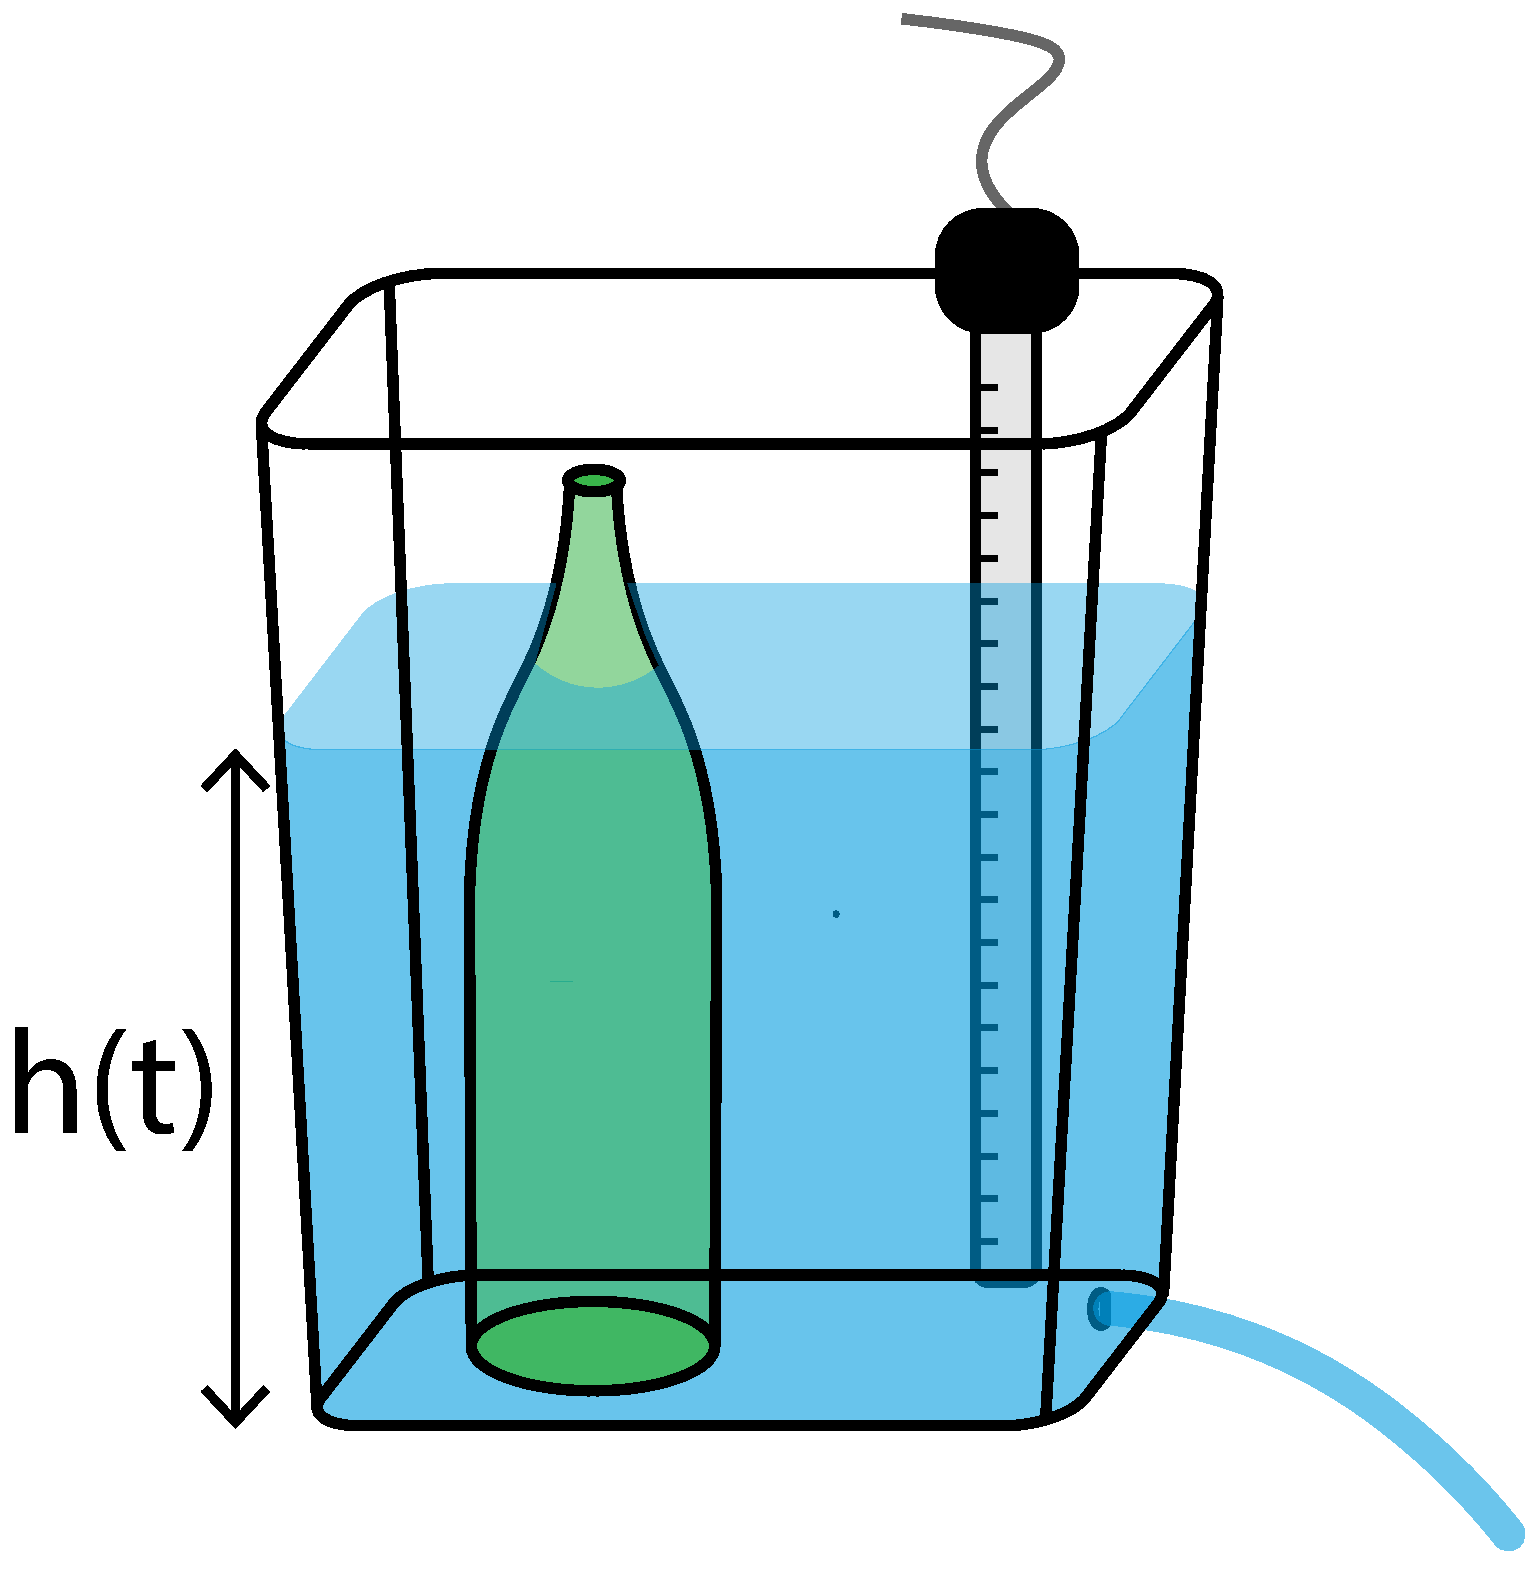
\includegraphics[width=\textwidth]{../tank_geometry/tank_w_bottle.pdf}
	\caption{Experimental setup} \label{fig:tank_w_bottle}
    \end{subfigure}
     \begin{subfigure}[b]{0.49\textwidth}
    	\includegraphics[width=\textwidth]{../prior_area.pdf}
	\caption{Prior dist'n of $\alpha(h)$} \label{fig:prior_area}
    \end{subfigure}
    
     \begin{subfigure}[b]{0.49\textwidth}
    	\includegraphics[width=\textwidth]{../posterior_object.pdf}
	\caption{Data $\{(t_i, h_i)\}$ and posterior dist'n of $h(t)$} \label{fig:posterior_object}
    \end{subfigure}
    \begin{subfigure}[b]{0.49\textwidth}
    	\includegraphics[width=\textwidth]{../posterior_area.pdf}
	\caption{Posterior dist'n of $\alpha(h)$} \label{fig:posterior_area}
    \end{subfigure}

    \caption{
      \textbf{Inferring the shape of the object in the tank.} 
      (a) We fill our tank containing a large, heavy, glass bottle with water, then, at $t=0$, allow it to drain through the orifice in its side.
      (b) Samples of the object cross-sectional area $\mathbf{A}$ from the prior distribution, along with the cross-sectional area of the tank (gray) for perspective. 
      (c) Time series data \thedata from the tank drainage experiment and samples of water level trajectories \themodel from the posterior distribution $\pi_{\text{post}}(\thevars \mid \thedatanomath)$.
      (d) Samples of the object cross-sectional area $\mathbf{A}$ from the posterior distribution, along with the cross-sectional area of the tank (gray) for perspective and the measured (held-out) cross-sectional area of the bottle inside the tank. 
      }
\end{figure}

\section{Conclusions and Discussion}
In phase I, we constructed, Bayesian-calibrated, and tested a forward model for the dynamics of the liquid level in our tank draining of water through a small orifice in its side---without an exogenous solid object inside the tank.
The calibrated model predicted the liquid level trajectory in our tank in a replicate experiment with a mean absolute residual of 0.28\,cm.
In phase II, we exploited our Bayesian-calibrated forward model to reconstruct the shape of a heavy, solid object (a bottle) inside the tank, using water level time series data as the tank containing the object drains of water. Essentially, the water ``scanned'' the area of the object as a function of its height as the tank drained. 
The range of the posterior distribution of the bottle's area as a function of height agreed reasonably well with our measurements of its area (mean absolute residual of 7.2\,cm$^2$) but exhibited a little bias. 
In conclusion, a forward model of the dynamics of the liquid level in a draining tank that contains a solid object, a probabilistic measurement model of the liquid level sensor, and liquid level time series data during the process of draining allow us to infer the area of the object as a function of height with quantified uncertainty via Bayesian statistical inversion. 

Our methods herein could be employed throughout engineering and the applied sciences, where one wishes to determine the shape of an object inside of an opaque liquid-holding tank with access to liquid level measurements.
More, one could infer the height or porosity of small, heavy solid particles (e.g. gravel, sand) packed into a liquid holding tank in a similar manner. 

\paragraph{Model calibration with an object in the tank.}
While we calibrated our model with tank draining experiments where the tank certainly did not contain an exogenous solid object inside of it, one could instead calibrate the model with an object inside the tank---provided the area of that object as a function of height is known. 

\paragraph{Alternative parameterizations of the object's shape.}
While we parameterized the area of the object as a function of height via the weights on triangle hat basis functions (see eqn.~\ref{eq:alpha_basis}), we could have instead (a) employed different basis functions or (b) if we knew the object's shape belonged to a certain category, adopted a more specific parameterization.
Route (a) may complicate expressing a prior distribution over the object's shape. 
To exemplify route (b), suppose we know the object is a triaxial ellipsoid. Then, we could parameterized the shape of the object by the lengths $a$, $b$, and $c$ of its principal axes.

\paragraph{Extensions.}
Our forward model of the dynamics of the liquid level in an \emph{open-top} tank, containing a solid, draining of liquid through a \emph{small} orifice in its side \emph{without} additional input/output of liquid could be extended to handle 
(a) closed tanks, where the air pressure in the headspace is not constant during draining; 
(b) larger orifices, where Torricelli's law does not hold and perhaps the liquid at the top does not remain flat;
and
(c) additional inputs/outputs of liquid by adding source/sink terms.
Note, (b) may necessitate modeling the flow streamlines inside the tank (as in Refs.~\cite{mathew2014numerical,sakri2017numerical}).
More, during the Bayesian calibration phase, we could learn a model discrepancy \cite{brynjarsdottir2014learning,kennedy2001bayesian} function to capture any bias---i.e., a difference between the true dynamics of the liquid level in the tank and the model $h(t; h_0^*,  \boldsymbol \alpha^*, \boldsymbol \theta^*)$ with the true/best-fit (indicated by $*$) initial water level, object geometry, and parameters.
% In other words, we assume our forward model is capable of capturing the true liquid level dynamics in the tank without bias.




% Mariotte's bottle \cite{kirevs2006mariotte}


\enlargethispage{20pt}

\ack{CMS acknowledges Intel. GF acknowledges ARMI for funding.}


\vskip2pc


\bibliographystyle{RS} %%%% .BST file

\bibliography{refs} %%%%% .Bib file

\end{document}
